\documentclass[trucol]{trucolpitchdeck}
\usepackage{amsmath} % need to be on top for eps files
\usepackage{caption}
\usepackage{subcaption}
\usepackage{graphicx}
\graphicspath{{latex/Images/}}
\usepackage{epstopdf}
\usepackage{svg}

%\usepackage[official]{eurosym}
%\usepackage{libertine}
\usepackage{textcomp}
\usepackage{eurosym}

\newcommand{\meuro}{\text{\euro}}
\makeatletter
% Definition taken from eurosym.sty, provides \EUR equivalent for math mode
\newcommand\MEUR[1]{\if@EURleft\text{\euro}\,\fi#1\if@EURleft\else\,\text{\euro}\fi}
\makeatother

%%%%%%%%%Custom
% Allow linking in document.
\usepackage{hyperref}

% Allow including autogenerated LaTex tables from Python.
\usepackage{booktabs}
\usepackage{longtable}
\usepackage{lipsum}

% Determine whether it is local compilation or overleaf compilation
\makeatletter
\begingroup\endlinechar=-1\relax
       \everyeof{\noexpand}%
       \edef\x{\endgroup\def\noexpand\homepath{%
         \@@input|"kpsewhich --var-value=HOME" }}\x
\makeatother
\def\overleafhome{/tmp}% change as appropriate


% Specify compilation name.
\def\filename{main}

% Specify what types of appendices are included in file.
\def\appendixtypes{no_code}
%\def\appendixtypes{project_code_only}
%\def\appendixtypes{export_code}
%\def\appendixtypes{project_and_export_code}



% Use H option in figure placement:
\usepackage{float}

% Use math letters
\usepackage{amsmath} % need to be on top for eps files
\usepackage{mathtools}

% Used for image geometry (already included)
%\usepackage{graphicx}

% Support auto referencing
\usepackage{cleveref}

\crefname{lstlisting}{listing}{listings}
\Crefname{lstlisting}{Listing}{Listings}

% Specify bibliography style:
\usepackage{url}

%%%%%%%%%End Custom




\usepackage[utf8]{inputenc}
\usepackage{geometry}
 \geometry{
 a4paper,
 total={175mm,265mm},
 left=1in,
 top=1.7in,
 }

\usepackage{amsmath}%To be able to use split in equation


%%%% Include eps files:
\usepackage{amsmath} % need to be on top for eps files
\usepackage{graphicx}
%set the relative location for eps files
\graphicspath{ {/Images/} }
\usepackage{listings}
\usepackage{cleveref} %cleverref needs to stand below amsmath package.
\usepackage{graphicx}
\usepackage{float}
%\usepackage{hyperref}
\usepackage{url} %To be able to use url in references
\usepackage{graphicx}
\usepackage{tabularx} % in the preamble
\usepackage{wrapfig}

% To get side by side pictures:{
\usepackage{caption}
\usepackage{subcaption}
\usepackage{graphicx}




%%%%%%%%%%%%%%%%%%%%%%%%%%%%%%%%%%%%%%%%%%%%%%%%%% Create listings (Python)
% set code color pattern (for python)
% Default fixed font does not support bold face
\DeclareFixedFont{\ttb}{T1}{txtt}{bx}{n}{12} % for bold
\DeclareFixedFont{\ttm}{T1}{txtt}{m}{n}{12}  % for normal

% Custom colors
\usepackage{color}
\definecolor{deepblue}{rgb}{0,0,0.5}
\definecolor{deepred}{rgb}{0.6,0,0}
\definecolor{deepgreen}{rgb}{0,0.5,0}

\usepackage{listings}

% Python style for highlighting
\newcommand\pythonstyle{\lstset{
language=Python,
breaklines=true, % wrap lines
postbreak=\mbox{\textcolor{red}{$\hookrightarrow$}\space}, % wrap lines
basicstyle=\ttm,
otherkeywords={self},             % Add keywords here
keywordstyle=\ttb\color{deepblue},
emph={MyClass,__init__},          % Custom highlighting
emphstyle=\ttb\color{deepred},    % Custom highlighting style
stringstyle=\color{deepgreen},
frame=tb,                         % Any extra options here
showstringspaces=false            %
}}

% Python environment
\lstnewenvironment{python}[1][]
{
\pythonstyle
\lstset{#1}
}
{}

% Python for external files
\newcommand\pythonexternal[2][]{{
\pythonstyle
\lstinputlisting[#1]{#2}}}

% Python for inline
\newcommand\pythoninline[1]{{\pythonstyle\lstinline!#1!}}


% Include path to images
\graphicspath{{Images/}{latex/project1/}}

% Include pdf files in report
\usepackage{pdfpages}


\usepackage{cleveref} %cleverref needs to stand below amsmath package.
\usepackage{appendix}
\crefname{appsec}{Appendix}{Appendices} % refer to appendix as appendix iso as section (use with text in
%\title{}
%\subtitle{}
\title{Roadmap: TruCol\\\large A decentralised collaboration protocol for test-driven development}
%\author{Authors:\\a-t-0}



%\def\parent_subpath{/latex/project}% change as appropriate (depending on what Overleaf does)
\usepackage{xstring}


%\def\project_one{/project1}% change as appropriate
%enable multirple columns
\usepackage{multicol}
\usepackage{multirow}

\usepackage{currfile}
\usepackage{currfile-abspath}

% use sidewaysfigure
\usepackage{rotating}

\date{\today}
\begin{document}
\crefname{lstlisting}{listing}{listings}
\Crefname{lstlisting}{Listing}{Listings}


\maketitle
%\setcounter{chapter}{-1}

% Create abstract.
\ifx\homepath\overleafhome
    % Overleaf compilation.
    \vspace{-0.16cm}
\section{Challenge}
\vspace{-0.15cm}
While trying to set out a programming bounty to speed up the development of another company, we noticed most bounty platforms take a cut as middleperson. We wanted the person that solves our problem, to get the full reward.
 %\newpage
    \vspace{-0.16cm}
\section{Solution}
\vspace{-0.15cm}
Decentralisation eliminates intermediaries. So we assembled a team of students from Delft- \& Radboud University, and competed at the ETHDenver in 2021. There we developed the trustless collaboration protocol for test driven development. %This protocol has been presented on the Ethereum Conference 4 in Paris.
 %\newpage
    \vspace{-0.16cm}
\section{Market Opportunity}
\vspace{-0.15cm}
Our business model changes after reaching series B/C. We first build a database of task- \& solution pairs as consultants. Upon acquiring sufficient data, we intend to pivot to TTD market making using an arbitrage bot built on that dataset.

\noindent The logistics market is good starting point due our affinity with its algorithmic and efficiency driven nature. Our top-down market analysis [Right QR] contains a Monte-Carlo simulation of the total addressable market size for the TruCol company. This TAM yields an estimated yearly revenue of 600K to 14M per year.
 %\newpage
  	\vspace{-0.16cm}
\section{Competition}
\vspace{-0.15cm}
In business model I, our competition consists of GitCoin, which take a 10\% cut and allow for ambiguity. We take no cut, and earn income by helping companies safely offload their tasks into the TruCol protocol. Additionally, we can facilitate companies in privacy-friendly, automated compliance using self-sovereign identities.

\noindent In business model II, our competition currently consists of GPT-4 and GitHub co-pilot, we expect this market to be so large that new competitors will come and go. We hope our headstart in this market will enable us to maintain a competitive edge.
 %\newpage
    \vspace{-0.16cm}
\section{Market Strategy}
\vspace{-0.15cm}
We aim to collaborate with 1 leading edge algorithmic firm, such as Optiver, to demonstrate the power of the TruCol protocol. If such a demonstration is successful, a rational market will follow. If the market is irrational, we will put in more effort to stimulate the usage of the TruCol protocol. [Roadmap: left QR]
 %\newpage
  	\vspace{-0.16cm}
\section{Team \& Impact}
\vspace{-0.15cm}
During the ETHDenver we learned about the profound impact of our protocol. It eliminates hiring bias, providing fair and inclusive work for all. On top of that, companies automatically get the lowest labour costs in the world, with solutions that are delivered on time with insurance.
\begin{figure}[htp]

    \centering
    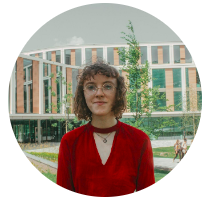
\includegraphics[width=.15\textwidth]{latex/Images/Clara.png}\hfill
    
\includegraphics[width=.15\textwidth]{latex/Images/Rashim.png}\hfill
    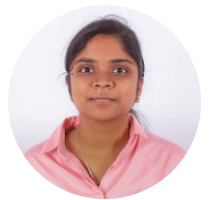
\includegraphics[width=.15\textwidth]{latex/Images/Subhechha.png}

    \caption*{We had a lot of fun in our journey with TruCol so far, thanks to the help of our team members with excellent communication and coding skills.}
    %\label{fig:figure3}

\end{figure}
 %\newpage
  	%\section{Introduction}
%
\hspace{11.5cm}\href{https://www.TruCol.io}{TruCol.io}%\newline
%\hspace{6cm}\href{https://github.com/TruCol/Roadmap/blob/main/main.pdf}{}
%\vspace{-1cm}
%\hspace{7cm}\href{https://github.com/TruCol/Market_analysis/blob/main/TruCol_market_analysis.pdf}{Market Analysis \& Roadmap (QRs):}

\begin{figure}[H]
    \vspace{-6cm}
    \hspace{13.5cm}
    
\includegraphics[width=0.08\textwidth]{latex/Images/roadmap.jpg}
    
\includegraphics[width=0.08\textwidth]{latex/Images/market_anlaysis.png}
\end{figure}


%amzqr https://github.com/TruCol/Market_analysis/blob/main/TruCol_market_analysis.pdf   -n github_qr.jpg
%amzqr https://github.com/TruCol/Market_analysis/blob/main/TruCol_market_analysis.pdf -c -con 1.5 -bri 1.6  -n github_qr.jpg
%amzqr https://github.com/TruCol/Market_analysis/blob/main/TruCol_market_analysis.pdf -p github.jpg -c -con 1.5 -bri 1.6

%amzqr https://github.com/TruCol/Roadmap/blob/main/main.pdf   -n roadmap.jpg
 %\newpage
\else
    % Local compilation
    \vspace{-0.16cm}
\section{Challenge}
\vspace{-0.15cm}
While trying to set out a programming bounty to speed up the development of another company, we noticed most bounty platforms take a cut as middleperson. We wanted the person that solves our problem, to get the full reward.
 %\newpage
    \vspace{-0.16cm}
\section{Solution}
\vspace{-0.15cm}
Decentralisation eliminates intermediaries. So we assembled a team of students from Delft- \& Radboud University, and competed at the ETHDenver in 2021. There we developed the trustless collaboration protocol for test driven development. %This protocol has been presented on the Ethereum Conference 4 in Paris.
 %\newpage
    \vspace{-0.16cm}
\section{Market Opportunity}
\vspace{-0.15cm}
Our business model changes after reaching series B/C. We first build a database of task- \& solution pairs as consultants. Upon acquiring sufficient data, we intend to pivot to TTD market making using an arbitrage bot built on that dataset.

\noindent The logistics market is good starting point due our affinity with its algorithmic and efficiency driven nature. Our top-down market analysis [Right QR] contains a Monte-Carlo simulation of the total addressable market size for the TruCol company. This TAM yields an estimated yearly revenue of 600K to 14M per year.
 %\newpage
  	\vspace{-0.16cm}
\section{Competition}
\vspace{-0.15cm}
In business model I, our competition consists of GitCoin, which take a 10\% cut and allow for ambiguity. We take no cut, and earn income by helping companies safely offload their tasks into the TruCol protocol. Additionally, we can facilitate companies in privacy-friendly, automated compliance using self-sovereign identities.

\noindent In business model II, our competition currently consists of GPT-4 and GitHub co-pilot, we expect this market to be so large that new competitors will come and go. We hope our headstart in this market will enable us to maintain a competitive edge.
 %\newpage
    \vspace{-0.16cm}
\section{Market Strategy}
\vspace{-0.15cm}
We aim to collaborate with 1 leading edge algorithmic firm, such as Optiver, to demonstrate the power of the TruCol protocol. If such a demonstration is successful, a rational market will follow. If the market is irrational, we will put in more effort to stimulate the usage of the TruCol protocol. [Roadmap: left QR]
 %\newpage
  	\vspace{-0.16cm}
\section{Team \& Impact}
\vspace{-0.15cm}
During the ETHDenver we learned about the profound impact of our protocol. It eliminates hiring bias, providing fair and inclusive work for all. On top of that, companies automatically get the lowest labour costs in the world, with solutions that are delivered on time with insurance.
\begin{figure}[htp]

    \centering
    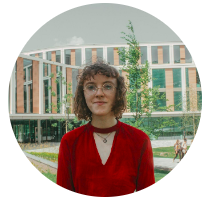
\includegraphics[width=.15\textwidth]{latex/Images/Clara.png}\hfill
    
\includegraphics[width=.15\textwidth]{latex/Images/Rashim.png}\hfill
    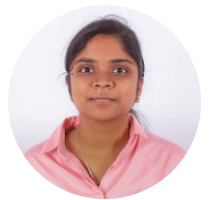
\includegraphics[width=.15\textwidth]{latex/Images/Subhechha.png}

    \caption*{We had a lot of fun in our journey with TruCol so far, thanks to the help of our team members with excellent communication and coding skills.}
    %\label{fig:figure3}

\end{figure}
 %\newpage
  	%\section{Introduction}
%
\hspace{11.5cm}\href{https://www.TruCol.io}{TruCol.io}%\newline
%\hspace{6cm}\href{https://github.com/TruCol/Roadmap/blob/main/main.pdf}{}
%\vspace{-1cm}
%\hspace{7cm}\href{https://github.com/TruCol/Market_analysis/blob/main/TruCol_market_analysis.pdf}{Market Analysis \& Roadmap (QRs):}

\begin{figure}[H]
    \vspace{-6cm}
    \hspace{13.5cm}
    
\includegraphics[width=0.08\textwidth]{latex/Images/roadmap.jpg}
    
\includegraphics[width=0.08\textwidth]{latex/Images/market_anlaysis.png}
\end{figure}


%amzqr https://github.com/TruCol/Market_analysis/blob/main/TruCol_market_analysis.pdf   -n github_qr.jpg
%amzqr https://github.com/TruCol/Market_analysis/blob/main/TruCol_market_analysis.pdf -c -con 1.5 -bri 1.6  -n github_qr.jpg
%amzqr https://github.com/TruCol/Market_analysis/blob/main/TruCol_market_analysis.pdf -p github.jpg -c -con 1.5 -bri 1.6

%amzqr https://github.com/TruCol/Roadmap/blob/main/main.pdf   -n roadmap.jpg
 %\newpage
\fi

% Include bibliography
%\bibliographystyle{plain} %plain style
%\bibliography{references}
%\addcontentsline{toc}{chapter}{Bibliography}

% Include appendices
\ifnum\pdfstrcmp{no_code}{\appendixtypes}=0
  % Don't include any code appendices. Feel free to add manual appendices here.
  \newpage
  \begin{appendices}
    \ifx\homepath\overleafhome
        % Overleaf compilation.
        %\input{Appendices/A_model_specification.tex} \newpage
 %\newpage
    \else
        % Local compilation
        %\input{latex/Appendices/A_model_specification.tex} \newpage
 %\newpage
    \fi
  \end{appendices}
\fi

% Include project code only.
\ifnum\pdfstrcmp{project_code_only}{\appendixtypes}=0
  \newpage
  \begin{appendices}
    \ifx\homepath\overleafhome
        % Overleaf compilation.
        \input{Appendices/Auto_generated_project_code_appendix___main__.tex} \newpage
\input{Appendices/Auto_generated_project_code_appendix_arg_parser.tex} \newpage
 %\newpage
    \else
        % Local compilation
        %\input{latex/Appendices/Auto_generated_project_code_appendix___main__.tex} \newpage
%\input{latex/Appendices/Auto_generated_project_code_appendix_arg_parser.tex} \newpage
 %\newpage
    \fi
  \end{appendices}
\fi

% Include only the code used to export the images, code etc. Skip project code.
\ifnum\pdfstrcmp{export_code}{\appendixtypes}=0
  \newpage
  \begin{appendices}
    \ifx\homepath\overleafhome
        % Overleaf compilation.
        \input{Appendices/Auto_generated_export_code_appendix_Hardcoded_data.tex} \newpage
\input{Appendices/Auto_generated_export_code_appendix_Plot_to_tex.tex} \newpage
\input{Appendices/Auto_generated_export_code_appendix_create_dynamic_diagrams.tex} \newpage
\input{Appendices/Auto_generated_export_code_appendix_create_static_diagrams.tex} \newpage
\input{Appendices/Auto_generated_export_code_appendix_export_data.tex} \newpage
\input{Appendices/Auto_generated_export_code_appendix_helper_bash_commands.tex} \newpage
\input{Appendices/Auto_generated_export_code_appendix_helper_dir_file_edit.tex} \newpage
\input{Appendices/Auto_generated_export_code_appendix_helper_tex_editing.tex} \newpage
\input{Appendices/Auto_generated_export_code_appendix_helper_tex_reading.tex} \newpage
\input{Appendices/Auto_generated_export_code_appendix_latex_compile.tex} \newpage
\input{Appendices/Auto_generated_export_code_appendix_latex_export_code.tex} \newpage
\input{Appendices/Auto_generated_export_code_appendix_plantuml_compile.tex} \newpage
\input{Appendices/Auto_generated_export_code_appendix_plantuml_generate.tex} \newpage
\input{Appendices/Auto_generated_export_code_appendix_plantuml_get_package.tex} \newpage
\input{Appendices/Auto_generated_export_code_appendix_plantuml_to_tex.tex} \newpage
 %\newpage
    \else
        % Local compilation
        \input{Appendices/Auto_generated_export_code_appendix_Hardcoded_data.tex} \newpage
\input{Appendices/Auto_generated_export_code_appendix_Plot_to_tex.tex} \newpage
\input{Appendices/Auto_generated_export_code_appendix_create_dynamic_diagrams.tex} \newpage
\input{Appendices/Auto_generated_export_code_appendix_create_static_diagrams.tex} \newpage
\input{Appendices/Auto_generated_export_code_appendix_export_data.tex} \newpage
\input{Appendices/Auto_generated_export_code_appendix_helper_bash_commands.tex} \newpage
\input{Appendices/Auto_generated_export_code_appendix_helper_dir_file_edit.tex} \newpage
\input{Appendices/Auto_generated_export_code_appendix_helper_tex_editing.tex} \newpage
\input{Appendices/Auto_generated_export_code_appendix_helper_tex_reading.tex} \newpage
\input{Appendices/Auto_generated_export_code_appendix_latex_compile.tex} \newpage
\input{Appendices/Auto_generated_export_code_appendix_latex_export_code.tex} \newpage
\input{Appendices/Auto_generated_export_code_appendix_plantuml_compile.tex} \newpage
\input{Appendices/Auto_generated_export_code_appendix_plantuml_generate.tex} \newpage
\input{Appendices/Auto_generated_export_code_appendix_plantuml_get_package.tex} \newpage
\input{Appendices/Auto_generated_export_code_appendix_plantuml_to_tex.tex} \newpage
 %\newpage
    \fi
  \end{appendices}
\fi

% Include project code and the code used to export the images, code etc.
\ifnum\pdfstrcmp{project_and_export_code}{\appendixtypes}=0
  \newpage
  \begin{appendices}
    \ifx\homepath\overleafhome
        % Overleaf compilation.
        \input{Appendices/Auto_generated_project_code_appendix___main__.tex} \newpage
\input{Appendices/Auto_generated_project_code_appendix_arg_parser.tex} \newpage
 %\newpage
        \input{Appendices/Auto_generated_export_code_appendix_Hardcoded_data.tex} \newpage
\input{Appendices/Auto_generated_export_code_appendix_Plot_to_tex.tex} \newpage
\input{Appendices/Auto_generated_export_code_appendix_create_dynamic_diagrams.tex} \newpage
\input{Appendices/Auto_generated_export_code_appendix_create_static_diagrams.tex} \newpage
\input{Appendices/Auto_generated_export_code_appendix_export_data.tex} \newpage
\input{Appendices/Auto_generated_export_code_appendix_helper_bash_commands.tex} \newpage
\input{Appendices/Auto_generated_export_code_appendix_helper_dir_file_edit.tex} \newpage
\input{Appendices/Auto_generated_export_code_appendix_helper_tex_editing.tex} \newpage
\input{Appendices/Auto_generated_export_code_appendix_helper_tex_reading.tex} \newpage
\input{Appendices/Auto_generated_export_code_appendix_latex_compile.tex} \newpage
\input{Appendices/Auto_generated_export_code_appendix_latex_export_code.tex} \newpage
\input{Appendices/Auto_generated_export_code_appendix_plantuml_compile.tex} \newpage
\input{Appendices/Auto_generated_export_code_appendix_plantuml_generate.tex} \newpage
\input{Appendices/Auto_generated_export_code_appendix_plantuml_get_package.tex} \newpage
\input{Appendices/Auto_generated_export_code_appendix_plantuml_to_tex.tex} \newpage
 %\newpage
    \else
        % Local compilation
        %\input{latex/Appendices/Auto_generated_project_code_appendix___main__.tex} \newpage
%\input{latex/Appendices/Auto_generated_project_code_appendix_arg_parser.tex} \newpage
 %\newpage
        \input{latex/Appendices/Auto_generated_export_code_appendix_Hardcoded_data.tex} \newpage
\input{latex/Appendices/Auto_generated_export_code_appendix_Plot_to_tex.tex} \newpage
\input{latex/Appendices/Auto_generated_export_code_appendix_create_dynamic_diagrams.tex} \newpage
\input{latex/Appendices/Auto_generated_export_code_appendix_create_static_diagrams.tex} \newpage
\input{latex/Appendices/Auto_generated_export_code_appendix_export_data.tex} \newpage
\input{latex/Appendices/Auto_generated_export_code_appendix_helper_bash_commands.tex} \newpage
\input{latex/Appendices/Auto_generated_export_code_appendix_helper_dir_file_edit.tex} \newpage
\input{latex/Appendices/Auto_generated_export_code_appendix_helper_tex_editing.tex} \newpage
\input{latex/Appendices/Auto_generated_export_code_appendix_helper_tex_reading.tex} \newpage
\input{latex/Appendices/Auto_generated_export_code_appendix_latex_compile.tex} \newpage
\input{latex/Appendices/Auto_generated_export_code_appendix_latex_export_code.tex} \newpage
\input{latex/Appendices/Auto_generated_export_code_appendix_plantuml_compile.tex} \newpage
\input{latex/Appendices/Auto_generated_export_code_appendix_plantuml_generate.tex} \newpage
\input{latex/Appendices/Auto_generated_export_code_appendix_plantuml_get_package.tex} \newpage
\input{latex/Appendices/Auto_generated_export_code_appendix_plantuml_to_tex.tex} \newpage
 %\newpage
    \fi
  \end{appendices}
\fi

\end{document}
